\section{Workflow}
\label{sec:workflow}

\subsection{Erläuterung}
\label{sec:workflow.erlaeuterung}
Wie bereits in Kapitel \ref*{sec:einfuehrung.grundbegriffe} erwähnt, ist ein dezentrales Versionskontrollsystem. Dadurch ist jeder Nutzer in der Lage ohne Abhängigkeit zu einem Server seinen Quellcode zu versionieren.

Jeder Nutzer kann sein eigenes Projekt durch \textit{git init} zu einem Git Repository initialisieren oder ein bestehendes Repository aus einem Online-Verzeichnis klonen. Beim klonen des Repositories wird der komplette Hierarchiebaum bzw. die Chronik mit jedem Commit und Branch geklont. Beim initialisieren eines neuen Repositories ist der Hierarchiebaum leer und unbeschrieben. Die Initialisierung eines neues Repositories wird bevorzugt beim neuen Projekten.

Um jedoch einen Workflow einzurichten, der es ermöglicht an bestehenden Projekten teil zu nehmen, muss zuerst das Projekt auf das lokale System geklont werden. Nachdem das Projekt als Git Repository auf dem lokalen System vorhanden ist, können Änderungen am Quellcode vorgenommen werden und in den Hierarchiebaum bzw. dem Repository hinzugefügt werden. Ist der Entwickler der Meinung, das alle Änderungen abgeschlossen sind, obliegt ihm selbst ob er seine Änderungen an den Hauptverantwortlichen einreicht. 

Der Entwickler kann seine Änderungen als Patch per E-Mail einreichen, sofern die Hauptverantwortlichen des geklonten Projekts dieses Verfahren unterstützen. Die bevorzugte Methode ist bei den meisten Online-Plattformen jedoch der Merge Request, manchmal auch Pull-Request genannt. 

Bei einem Merge-Request fragt man an, ob eine bestimmte Sammlung von Commits, die eine Änderung des Quellcodes wieder spiegeln, durch die Hauptverantwortlichen übernommen werden. Dadurch wird der Hierarchiebaum des Online-Repositories um die eigenen Commits erweitert. Anderen Entwickler, die auch dieses Repository geklont haben, können zukünftig die Änderung aus dem Online-Repository auf ihr eigenes lokales Repository übernehmen.

\begin{figure}[h]
  \centering
  \label{img:workflow}
  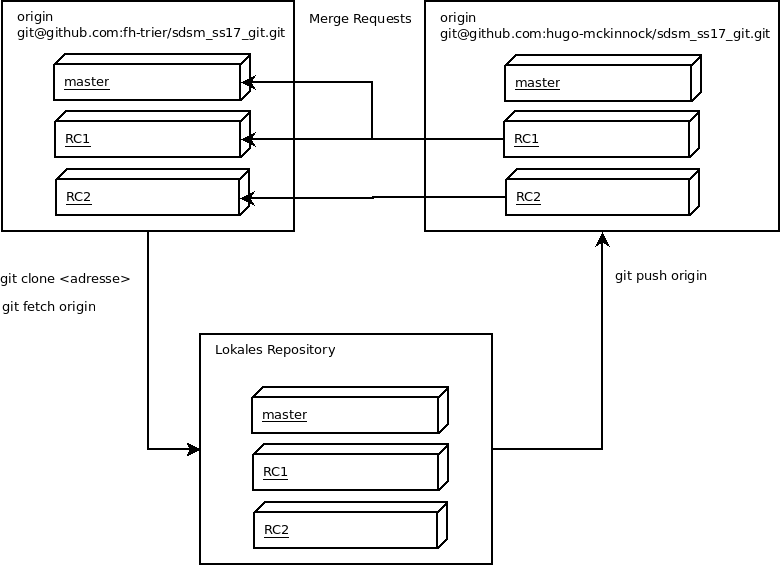
\includegraphics[width=1\textwidth]{images//workflow.png}
  \caption{Workflow}
\end{figure}  


\subsection{Einrichtung}
\label{sec:workflow.einrichtung}
Im Heimatverzeichnis wird wie von vielen IDE's bevorzugt, das Verzeichnis \textit{workspace} erstellt. Dort wird von dem Online-Repository \href{https://github.com}{GitHub} dieses \LaTeX{} Projekt, das dieses Dokument enthält, geklont. Nach dem klonen befindet sich im Verzeichnis \textit{workspace} der Unterordner \textit{sdsm\_ss17\_git}, in den mittels \textit{cd} nachträglich navigiert wird.

\begin{minted}[framesep=2mm, fontsize=\small]{bash}
$ mkdir ~/workspace
$ git clone git@github.com:fh-trier/sdsm_ss17_git.git
$ cd sdsm_ss17_git
\end{minted}

\begin{INFO}
  Zum klonen eines Online-Repositories wird auf vielen Online-Plattformen wie \href{https://github.com}{GitHub} oder \href{https://gitlab.com}{GitLab} eine Adresse per \textit{HTTPS-} oder \textit{SSH-}Protokoll angeboten. 
  
  Für eine Verbindung per SSH-Protokoll muss ein Account auf diesen Online-Plattformen registriert und der öffentliche Schlüssel des asymmetrischen Verschlüsselungsverfahren hinterlegt sein.  
\end{INFO}

Das heruntergeladene Repository spiegelt nun den Zustand wieder, auf dem sich die Referenz \textit{HEAD} befindet. Um dies zu überprüfen, bietet Git den Befehl \textit{git log} an. Wir lassen uns die neusten zwei Commits anzeigen.

\begin{minted}[framesep=2mm, fontsize=\small]{bash}
$ git log -2
commit e42f6e04ac8c3d2cf7d1e2c3b5dd5f7257612dc5 (HEAD -> master, origin/master)
Author: Markus Pesch <markus.pesch@cryptic.systems>
Date:   Thu Mar 15 21:59:24 2018 +0100

fix: chapter 2.2

commit 800ac8b5930ebe0650b83471aee957fe2195de05
Author: Markus Pesch <markus.pesch@cryptic.systems>
Date:   Thu Mar 15 21:53:14 2018 +0100

fix: chapter 2.
\end{minted}

Zu erkennen ist, dass sich die Referenz \textit{HEAD} auf der gleichen Position wie der Branch \textit{master} befindet. Der Branch \textit{master} ist ein Branch auf dem lokalen System des Entwicklers. Die Referenz \textit{origin/master} referenziert auf den Commit, auf dem das Online-Repository \textit{origin} und dessen Branch \textit{master} steht. Alle Referenzen referenzieren auf den Commit mit der ID \textit{e42f6e0}.

\begin{WARN}
  Zeigt \textit{HEAD} nicht auf einen Branch, spricht man davon, dass \textit{HEAD} losgelöst von einem Branch ist. Dies ist nur Sinnvoll um ältere Zustände zu betrachten, da auf einem losgelösten Zustand keine Änderungen angewandt werden können.
\end{WARN}

Um zu überprüfen welche Adresse sich hinter dem Label \textit{origin} befindet, bietet Git den Befehl \textit{git remote -v} an.

\begin{minted}[framesep=2mm, fontsize=\small]{bash}
$ git remote -v
origin  git@github.com:fh-trier/sdsm_ss17_git.git (fetch)
origin  git@github.com:fh-trier/sdsm_ss17_git.git (push)
\end{minted}

Zu erkennen ist, dass bei dem Befehl \textit{git fetch origin} alle neuen Commits von der Adresse \textit{git@github.com:fh-trier/sdsm\_ss17\_git.git} heruntergeladen werden - gekennzeichnet durch \textit{fetch}. Bei einem \textit{git push origin} versucht Git alle neuen Commits auf die gleiche Adresse, gekennzeichnet durch \textit{push}, zu schreiben. 

\begin{INFO}
  Lässt man das Label bei \textit{git fetch} und \textit{git push} weg, nimmt Git automatisch das Label \textit{origin} an. Das Label \textit{origin} ist das Standard-Label zur Bezeichnung von Remote-Adressen.
\end{INFO}

Möchte man nun seine Commits auf pushen, wird Git den push zurückweisen. Der Grund ist, dass man nicht der Eigentümer des Repositories unter der Adresse \textit{git@github.com:fh-trier/sdsm\_ss17\_git.git} ist. Um dies zu lösen, muss unter dem Label \textit{origin} die \textit{push}-Adresse geändert werden. Die einfachste Möglichkeit ist, sich auf der gleichen Online-Plattform, hier \href{https://github.com}{GitHub}, einen eigenen Benutzernamen zu registrieren und einen Ableger, auch Fork genannt, zu erzeugen. Man erhält anschließend eine neue Adresse, die den eigenen Benutzernamen enthält. 

Nun wird Git mitgeteilt, die neue Adresse als \textit{push}-Adresse unter dem Label \textit{origin} zu nutzen. Nach dem setzen werden die Adressen überprüft.

\begin{minted}[framesep=2mm, fontsize=\small]{bash}
$ git remote set-url origin \ 
      --add --push git@github.com:hugo-mckinnock/sdsm_ss17_git.git
$ git remote -v
origin	git@github.com:fh-trier/sdsm_ss17_git.git (fetch)
origin	git@github.com:hugo-mckinnock/sdsm_ss17_git.git (push)
\end{minted}

\begin{INFO}
  Möchte man sein Repository bei einem \textit{git push} Befehl auf mehrere Online-Repositories kopieren, dann kann der Befehl zum hinzufügen wiederholt werden unter Angabe einer weiteren Adresse.
\end{INFO}

Möchte man eine komplette Remote-Verbindung entfernen, kann dies unter Angabe des Git Befehls \textit{git remote remove  $ < $label $ > $} vorgenommen werden. 
  
Hinzufügen einer neuen Remote-Verbindungen ist möglich mit Angabe des neuen Labels mittels \textit{git remote add $ < $label$ > $ $ < $adresse$ > $}.

Nun ist der komplette Workflow eingerichtet und es wird Zeit sich mit den essentiellen Funktionen von Git zu beschäftigen. Dazu mehr in Kapitel 3.
